\section{Evaluation}
\label{sec.eval}
Our objective with this project was to \emph{explore if it is possible to abstract the creation of simple location-based systems from a programming level to a configuration level} and to \emph{discuss to what extent our system can support complex interactions between user and system}. To evaluate to what extend we have met this objective, we conducted an evaluation in three parts. First we evaluated the Realms configurator with users by having them configure a realm. Second, we evaluated the mobile client with users having to explore some predefined realms. These evaluations focussed on the investigating the balance between the expressiveness (the complexity of interactions we could support) and the usability.

\subsection{Participants} % (fold)
\label{sub:participants}
We recruited a total of 9 participants - 8 male and 1 female. All were students at the IT University of Copenhagen but included both undergraduate, master and phd students. Each participant was asked about age, and ask to rate their programming experience and mobile application mobile experience on a scale of 0 - 5 (0 for no experience, 5 for highly experienced). The average age of the participants was 26.67 (\sigma = 3.46). Their reported programming experience was 3.89 (\sigma = 1.26) and their reported mobile application programming experience 2.33 (\sigma =  1.41). 
% subsection participants (end)

\subsection{Procedure} % (fold)
\label{sub:procedure}
Each participant was given an introduction to the system as a general and was there after asked to try out one of the programs (configurator or mobile client). We switched the order in which the participants tried to the programs so 5 started with the configurator and 4 with the mobile client. Having tried the first program, the participants were interviewed regarding their experience before trying the second part of the system. Lastly, the participants were interviewed about the second part they tried a well as the the system as a whole. 
\\\\
While our system deals with user-profiles and requires a registration to use, we left this aspect out of the evaluation. Our focus was on the impression of the configurator and the mobile client. For all tests, the participants were logged in with one standard user.
\\\\
The interviews we conducted were semi-structured interviews that included question regarding the usefulness of the system, the expressiveness of the configurator and the usability of the configurator and client. Being semi-structured interviews, we let the participants talk as they wanted and encouraged them to say everything that came in to their minds. 
\\\\
We would have liked to do a comparative study where the participants would create a similar service to the one that they would configure in Realms. That process however, would have been time consuming as the only other way to our knowledge would be to program a new app that allows users to explore information and questions around a physical area. We therefore proceeded with a user-test of our system with no comparison to other methods.
\\\\
For the semi-structured interview we asked the participants the following questions:

\paragraph{Configurator specific questions} % (fold)
\label{par:configurator_specific_questiosn}
\begin{itemize}
	\item Do you see the creation of realms as useful?
	\item Do you feel the configurator provides enough options?
	\item Are there other features you would like to see?
	\item How was the usability?
\end{itemize}
% paragraph configurator_specific_questiosn (end)

\paragraph{Mobile client specific questions} % (fold)
\label{par:mobile_client_specific_questions}
\begin{itemize}
	\item How was the usability of the client?
	\item Did you find the client useful?
	\item Are there other features you would like to see?
\end{itemize}
% paragraph mobile_client_specific_questions (end)

The whole session, including the interviews lasted around 45 minutes.

\paragraph{Other questions} % (fold)
\label{par:other_questions}
\begin{itemize}
	\item (For people who tried the configurator first) How does exploring a Realm compare to the thought you had when creating a Realm?
	\item (For people who tried the mobile client first) Having tried the client first, were there any opportunities or limitations you thought about when configuring you own Realm?
	\item We use the notion of Realms to explain an augmented physical location. How does this notion fit with your experience of using the system.
\end{itemize}
% paragraph other_questions (end)
% subsection procedure (end)

\subsection{Scenarios} % (fold)
\label{sub:scenarios}
We gave the participants two scenarios - one for the configurator and one for the mobile client - that we asked them to play out. During the scenarios we observed the participants and helped when asked.

\subsubsection{Configurator} % (fold)
\label{sub:configuration_manager_evaluation}
For this test we created a scenario where users are asked to take on the position as a employee in the Copenhagen municipality. They were given the task to create a configuration to be used by tourist to explore the historical sites of Copenhagen. We asked the participants to create a Realm in Copenhagen and mark a few points of interest using both information and question markers.
\\\\
The participants were seated at a computer equipped with a 24\" widescreen - our current design is not well suited for low resolutions, so we decided to chose the hardware. We gave a short introduction to the system as a whole and showed users how to create a Realm and how to create marks. The participant was then asked to play out the scenario. In fig. \ref{fig:testing} a user is testing the configurator.

\begin{figure}
	\centering
	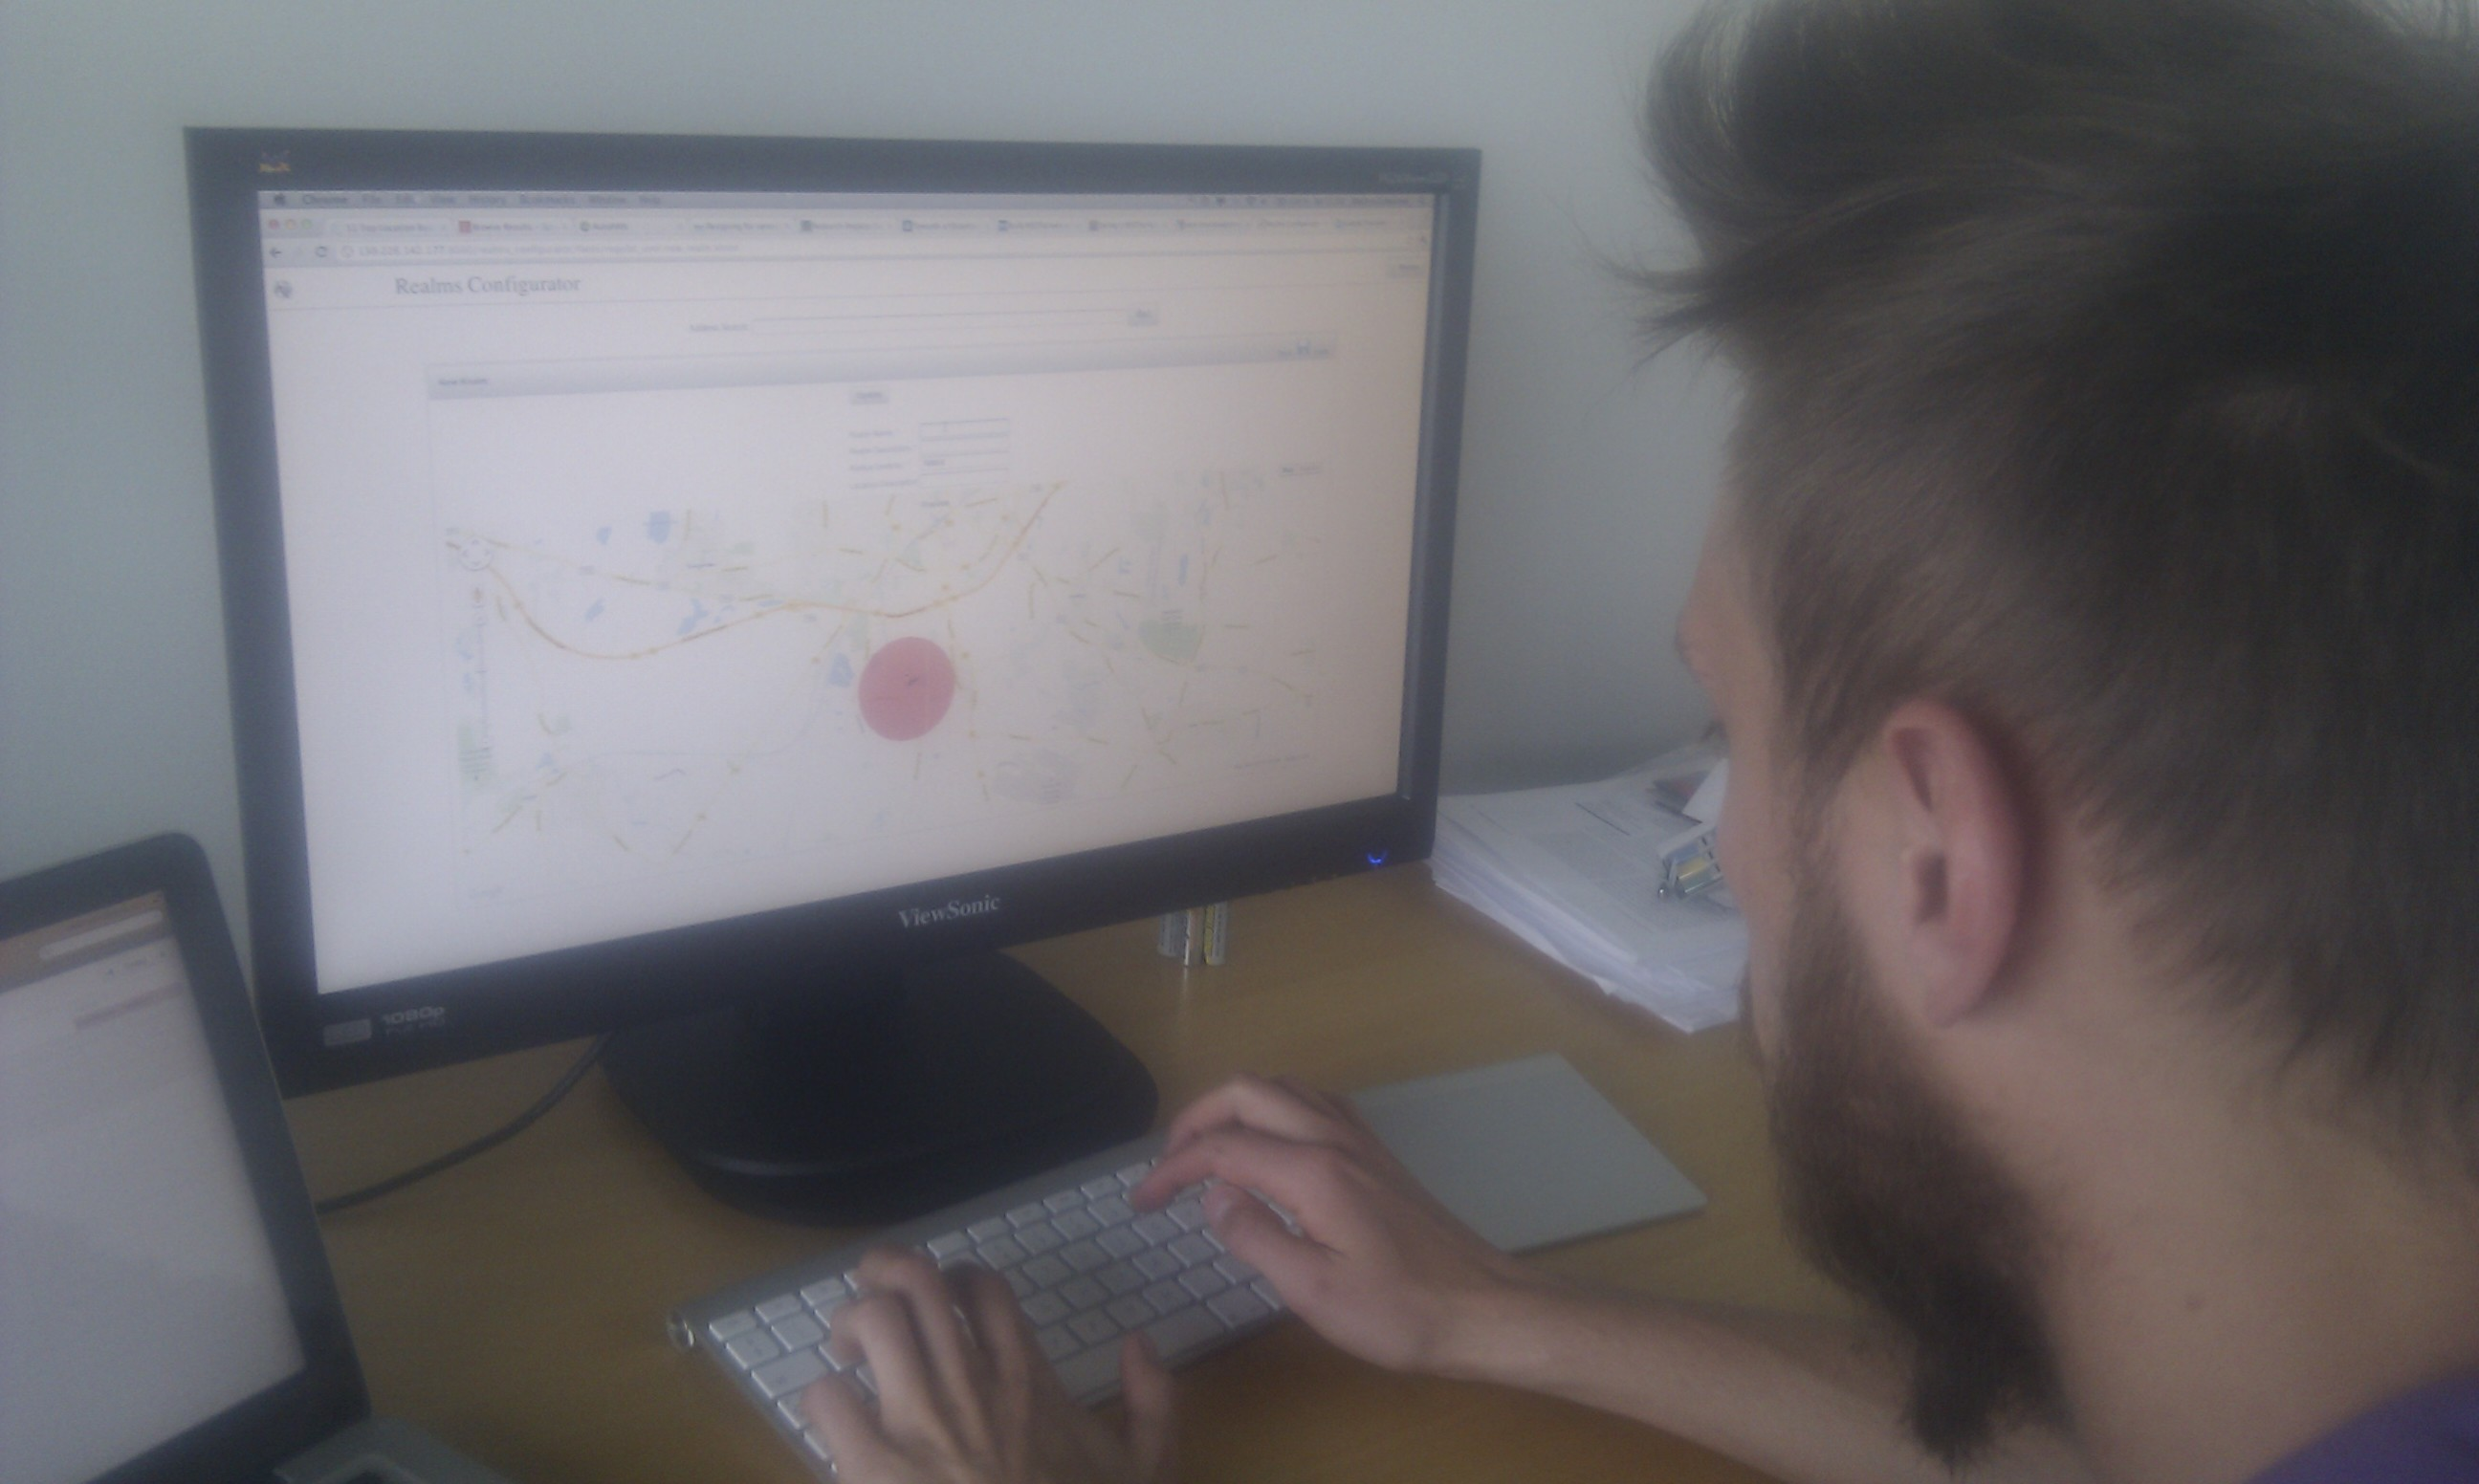
\includegraphics[scale=0.14]{fig/testing}
	\caption{A participant in our user trying the configurator}
	\label{fig:testing}
\end{figure}
% subsection configuration_manager_evaluation (end)

\subsubsection{Mobile Client} % (fold)
\label{sub:android_application_evaluation}
For the mobile application test we created a realm with the purpose of rating architecture around the city. The realm covered the IT University of Copenhagen as well as the surrounding building that include Copenhagen University buildings, an office building, a library, and a some student housings. For each of these buildings we created a marker with a either a description of the building, like year it was raised and the name of the architect who designed it, or a question regarding the history of the building or hosted institution. Our test users were given the task to go outside, enter the "Architecture Amager" realm, and walk around to different buildings in the area to explore the markers and rate them. The configuration for the Realm is shown in fig \ref{fig.amager.arc}.

\begin{figure}[ht]
	\centering
	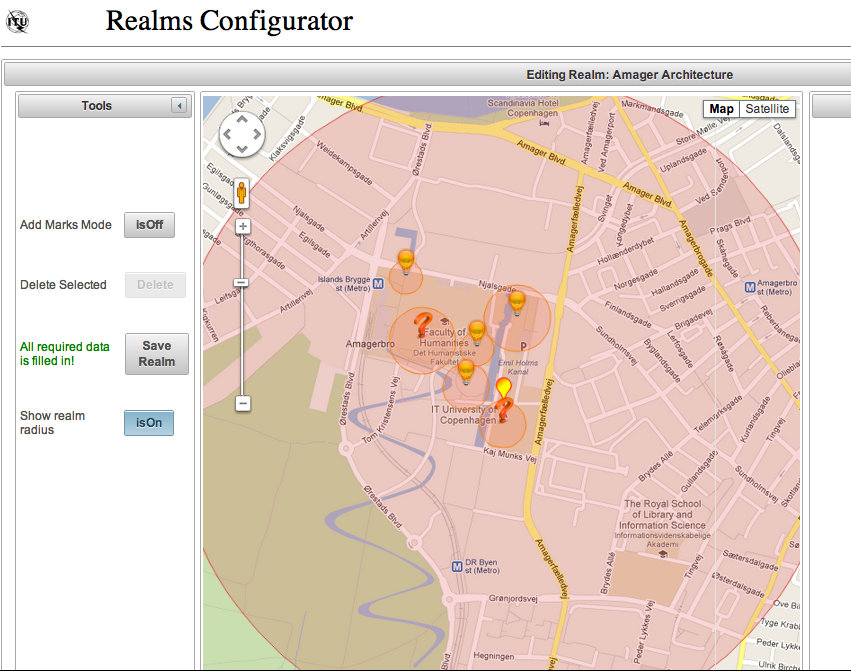
\includegraphics[scale=0.5]{fig/amager_configuration}
	\caption{Configuration for the test Realm Amager Architecture}
	\label{fig.amager.arc}
\end{figure}

\noinden We asked the participants to take a walk we us outside the university to play the scenario. The users were given a smartphone with the installed mobile application and GPS, Wifi and mobile data connection turned on. They were told that a Realm was available for them. They were also told in which direction to walk without telling them which buildings in that direction that were marked. We kept walking around until at least 3 markers had been discovered after which the participants were told that we could go back or continue around to find a few more markers if they preferred.
\\\\
In the next section we discuss the results of the evaluation.

% subsection android_application_evaluation (end)